The Input/Output layer is a client-side interface for the user to visualize the output of the drone detection and communicate with the drone detection system. The Input/Output layer has three subsystems: Results Display, User Inputs and Application.

\subsection{Results Page}
The results page includes the output of the drones detected in the area which is presented to the user in graphical form. 


\begin{figure}[h!]
	\centering
 	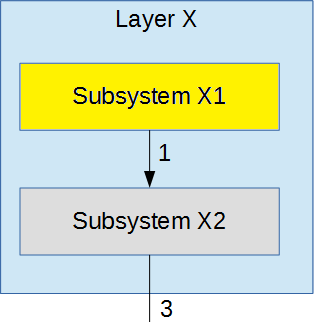
\includegraphics[width=0.60\textwidth]{images/subsystem}
 \caption{Example subsystem description diagram}
\end{figure}

\subsubsection{Assumptions}
The results page will only be online after the system is turned on.

\subsubsection{Responsibilities}
The responsibility of the results page is to provide a graphical visualization of the location of the system and any drones detected in the surrounding area communicating with the database from the application interface. The results page will display the location of the device in the form of circular dot and any detected drones will be shown in triangular shape.

\subsubsection{Subsystem Interfaces}

\begin {table}[H]
\caption {Results interfaces} 
\begin{center}
    \begin{tabular}{ | p{1cm} | p{6cm} | p{3cm} | p{3cm} |}
    \hline
    ID & Description & Inputs & Outputs \\ \hline
    \#U3 & Communication with the application & \pbox{3cm}{drones data from the database} & \pbox{3cm}{Graphical view of the detected drones}  \\ \hline
    \#U3 & Communication with application for system location & \pbox{3cm}{location data of the system} & \pbox{3cm}{Graphical view of the location of the system}  \\ \hline
    \end{tabular}
\end{center}
\end{table}

\subsection{User Inputs}
The User Inputs page includes the input that can be taken from the user. Here, the user can select a detected drone and verify that it is a false positive. Also, user can select an individual drone and the system will actively track the selected drone in as close to real time as possible.


\begin{figure}[h!]
	\centering
 	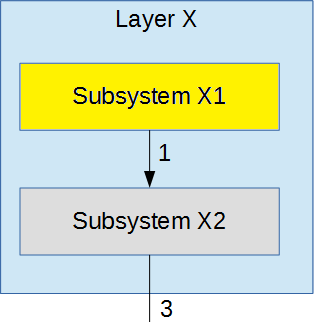
\includegraphics[width=0.60\textwidth]{images/subsystem}
 \caption{Example subsystem description diagram}
\end{figure}

\subsubsection{Assumptions}
The user can only select one drone at a time for active detection.

\subsubsection{Responsibilities}
The responsibility of the User Inputs is to provide a user interface to the user where they can select a detected drone and verify that it is a false positive, select an individual drone and the system will actively track the selected drone in as close to real time as possible.

\subsubsection{Subsystem Interfaces}

\begin {table}[H]
\caption {Subsystem interfaces} 
\begin{center}
    \begin{tabular}{ | p{1cm} | p{6cm} | p{3cm} | p{3cm} |}
    \hline
    ID & Description & Inputs & Outputs \\ \hline
    \#xx & Description of the interface/bus & \pbox{3cm}{input 1 \\ input 2} & \pbox{3cm}{output 1}  \\ \hline
    \#xx & Description of the interface/bus & \pbox{3cm}{N/A} & \pbox{3cm}{output 1}  \\ \hline
    \end{tabular}
\end{center}
\end{table}

\subsection{Application Subsystem}
The results page includes the output of the drones detected in the area which is presented to the user in graphical form. 


\begin{figure}[h!]
	\centering
 	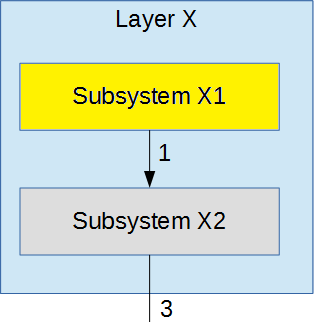
\includegraphics[width=0.60\textwidth]{images/subsystem}
 \caption{Example subsystem description diagram}
\end{figure}

\subsubsection{Assumptions}
The results page will only be online after the system is turned on.

\subsubsection{Responsibilities}
The responsibility of the results page is to provide a graphical visualization of the location of the system and any drones detected in the surrounding area. The results page will display the location of the device in the form of circular dot and any detected drones will be shown in triangular shape.

\subsubsection{Subsystem Interfaces}

\begin {table}[H]
\caption {Subsystem interfaces} 
\begin{center}
    \begin{tabular}{ | p{1cm} | p{6cm} | p{3cm} | p{3cm} |}
    \hline
    ID & Description & Inputs & Outputs \\ \hline
    \#01 & Drone False Positive & \pbox{3cm}{input 1 \\ input 2} & \pbox{3cm}{output 1}  \\ \hline
    \#xx & Description of the interface/bus & \pbox{3cm}{N/A} & \pbox{3cm}{output 1}  \\ \hline
    \end{tabular}
\end{center}
\end{table}


